\documentclass{bioinfo}
\usepackage{listings}
\usepackage{multirow}
%\usepackage{hyperref}
\copyrightyear{2014}
\pubyear{2014}


\lstset{
breaklines=true,	
}

\begin{document}
\firstpage{1}

\title[NxRepair]{NxRepair: Error correction in de novo sequence assembly using Nextera mate pairs}
\author[Murphy \textit{et~al}]{Rebecca R. Murphy\,$^{1}$, Jared O'Connell\,$^{1}$, Anthony J. Cox\,$^{1}$ and Ole Schulz-Trieglaff\,$^{1}$\footnote{to whom correspondence should be addressed}}
\address{$^{1}$Illumina Cambridge, Chesterford Research Park, Essex, CB10 1XL}

\history{Received on XXXXX; revised on XXXXX; accepted on XXXXX}

\editor{Associate Editor: XXXXXXX}

\maketitle

\begin{abstract}

\section{Motivation:}
Incorrect traversals of the de Bruijn graph during de novo assembly and scaffolding errors can result in large scale misassemblies in draft genomes. Nextera mate pair sequencing data provide additional information to resolve assembly ambiguities during scaffolding. We introduce a routine that uses mate-pair information to identify and correct large-scale errors in genome assemblies.    
\section{Results:}
We introduce NxRepair, a toolkit for error correction in de novo assemblies using Nextera mate pair libraries. We show that NxRepair can identify and correct large scaffolding errors, without use of a reference sequence, resulting in quantitative improvements in the assembly quality.
\section{Availability:}
NxRepair is open source software and is written in Python as both a suite of command line utilities and a Python application programming interface. It can be downloaded from GitHub at \href{https://github.com/rebeccaroisin/nxrepair}{https://github.com/rebeccaroisin/nxrepair}. User documentation and a tutorial are hosted at \href{http://nxrepair.readthedocs.org/}{http://nxrepair.readthedocs.org/}.
\section{Supplementary information:}
Supplementary figures and details of the genomes evaluated are available at \emph{Bioinformatics} online. 
\section{Contact:} \href{oschulz-trieglaff@illumina.com}{oschulz-trieglaff@illumina.com}
\end{abstract}

\section{Introduction}
De Bruijn Graph construction and traversal is a popular method for de novo genome assembly~\citep{compeau2012}. However, traversal of repeat regions, which tangle the de Bruijn Graph, remains challenging. Large-insert size read pairs, such as the Illumina Nextera mate pairs can provide additional information for repeat disambiguation. Many assemblers incorporate mate pair insert size information into the assembly and scaffolding process~\cite{bankevich2012, zerbino2008}, but large scale scaffolding errors can still occur (Fig.~\ref{fig:NxRepair} (A)). Here we introduce NxRepair, an assembly error detection tool that can identify the most serious misassemblies by examining the distribution of Nextera mate pair insert sizes, without using a reference sequence. NxRepair specifically targets the most serious misassemblies by identifying regions with a high number of anomalous insert sizes, breaking the scaffold and optionally trimming out the misassembled region. 

\begin{figure*}
\centerline{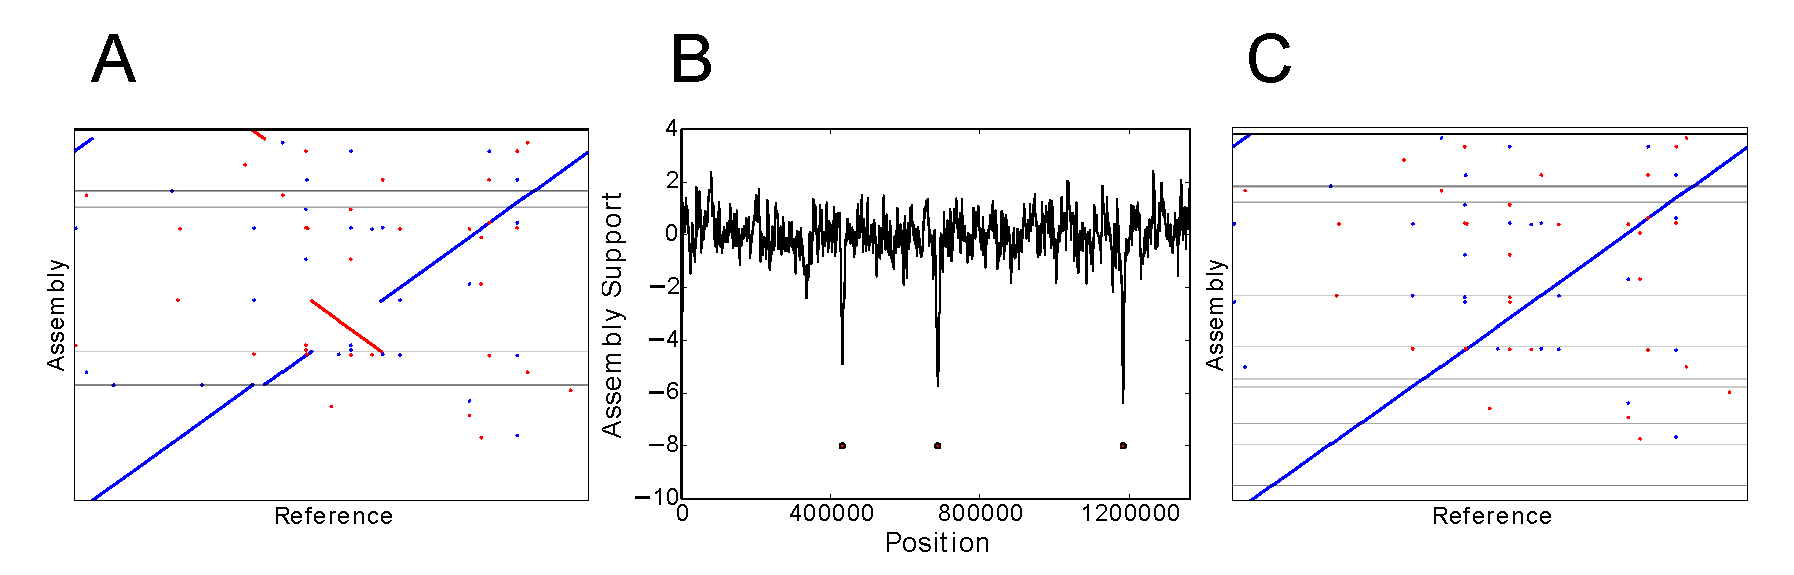
\includegraphics[width=0.8\textwidth]{fig1_nxrepair.pdf}}
\caption{Using NxRepair to remove large misassemblies. (A) A de novo assembly of the Mycobacterium tuberculosis genome contains several large misassemblies. (B) Low support for the assembly is identified in two regions using NxRepair. (C) Breaking the contigs at the identified positions resolves the most significant misassemblies. In (A) and (C), horizontal lines demarcate contig boundaries.}\label{fig:NxRepair}
\end{figure*}

\begin{table}[!t]
\processtable{Number of large misassemblies and NGA50 as reported by QUAST before and after NxRepair correction. \label{tab:improvement}}
{\begin{tabular}{lllllll}\toprule
 & \multicolumn{2}{l}{Before NxRepair} & \multicolumn{4}{l}{After NxRepair} \\\midrule
Genome & No. & NGA50 & No. & NGA50 \\\midrule
Bcer & 3 & 1157404 & 3 & 1157404 \\
EcDH & 8 & 576143 & 8 & 576143 \\
EcMG & 2 & 640732 & 2 & 640732 \\
List & 0 & 1496615 & 0 & 1496615 \\
Meio & 0 & 3095733 & 0 & 3095733 \\
ped & 6 & 1269259 & 0 & 1269259 \\
pneu & 7 & 577220 & 6 & 577220 \\
Rhod & 9 & 3181390 & 9 & 3181390 \\
TB & 70 & 184170 & 66 & 158885 \\\botrule
\end{tabular}}{}
\end{table}


\begin{methods}
\section{Methods}
\subsection{Statistical Analysis of Mate Pair Insert Sizes}
Nextera mate pair libraries are prepared to have a certain insert size, typically between 1 and 10 kb. When the mate pairs used to prepare an assembly are aligned back to the assembly, large misassemblies result in unusual insert sizes and read orientations. We model this using a two-component mixture distribution. The first component of this mixture is the insert size distribution of correctly aligned mate pairs.  We model the $\log$ of the insert sizes, say $Y$, as a normal distribution with mean $\mu$ and standard deviation $\sigma$: $Y \sim N(\mu,\sigma^2).$ Since assemblies are mostly correct, we can estimate $\mu$ and $\sigma$ by aligning reads back to the assembly and using robust estimators. The second component, defined as uniform across the contig size $U(0,L)$ for a contig of length $L$, captures anomalous insert sizes. We define a latent indicator variable $X_i\in\{0,1\}$ for the $i$th pair of reads that span position $l$, which takes the value $1$ if the insert size came from our null distribution, and $0$ otherwise.

For each mate pair, the posterior probability of $X_i$, given its insert size $Y_i$, is then:

\begin{eqnarray} P(X_i=x|Y_i)& =& \frac{P(X_i=x)(Y_i|X_i=x)}{\sum_{k=0}^1P(X_i=k)(Y_i|X_i=k)}\\
  & =& \frac{\pi_x(Y_i|X_i=x)}{\sum_{k=0}^1 \pi_k(Y_i|X_i=k)}
\label{eq:posterior}  
\end{eqnarray}

where $\pi_x$ is the prior probability of class $x$ and $\pi_1 + \pi_0 = 1$. For each position $l$ on the contig that is spanned by $N$ read pairs, the total support for a correct assembly at a particular assembly position is calculated as $D_l = \sum_{i=1}^N P(X_i=1|Y_i)\cdot C_i$ where $C_i$ is an indicator variable, reporting pairing orientation:

\begin{equation}
    C_i=
    \begin{cases}
      1, & \text{if}\ \text{read pair $i$ has correct orientation and strand alignment} \\ 
      0, & \text{otherwise}
    \end{cases}
  \label{eq:C}
  \end{equation}

Finally, having obtained a value of $D_l$ at sites $l = 1,\ldots,L$ across the assembly, we calculate a typical standard score ($Z_l$) to evaluate how extreme the value of $D_l$ is. Where

\begin{equation}
Z_l=\frac{D_l - \bar{d}}{s_D}
\label{eq:zscore}
\end{equation}

where $\bar{d}$ and $s_D$ are just standard the sample mean and standard deviation across all $L$ sites. For a user-defined threshold $T$, NxRepair will identify a misassembly if $Z_l < T$ and will break the contig into two pieces at the site identified  (default $T=-4$).

%% \begin{equation}
%% \bar{d}_D = \frac{\sum_{l=1}^L D_l}{L} \qquad s_D = \frac{\sum_{k=1}^L \sqrt{(D_k - \bar{d})^2}}{L - 1}
%% \end{equation}



\subsection{Usage}
NxRepair analysis requires the assembly in FASTA format and a sorted BAM file containing the same Nextera mate pair reads used in assembly aligned back to the assembly. NxRepair assembly correction can be performed in a single step and outputs a csv file containing the $Z$ score at each site evaluated; the repaired de novo assembly as a new fasta file; and, optionally, a series of graphs plotting the NxRepair $Z$ score and highlighting identified errors.   

\end{methods}


\section{Results and Discussion}
We used NxRepair to correct de novo assemblies from nine bacterial genomes. The genomes used are described in the supplementary information. Mate pair reads were trimmed, assembled using the SPAdes assembler (version 3.1.1)~\citep{bankevich2012} and then aligned back to the assembled scaffold using BWA-MEM~\citep{li2013}. We used QUAST~\citep{gurevich2013} to evaluate the assembly quality before and after NxRepair correction by aligning to an appropriate reference genome. Fig.~\ref{fig:NxRepair} (A) shows a misassembled genome that contained several scaffolding errors identified by NxRepair (Fig.~\ref{fig:NxRepair} (B)). Following NxRepair correction, the most significant structural misassemblies were resolved (Fig.~\ref{fig:NxRepair} (C)). The improvement following NxRepair correction is shown for all nine genomes in Table~\ref{tab:improvement}. For two assemblies, errors were removed without reducing NGA50; for one genome, errors were removed but NGA50 was slightly reduced; for five genomes, two of which contained no large errors, no errors were found and the assembly was unchanged.

\section{Conclusion}
NxRepair is a simple error correction module that can be used to identify and remove large scale errors from de novo assemblies using Nextera mate pair reads. The tool is freely available online and can be run with a single call from the command line, making it an attractive option for improving assembly quality.
\paragraph{Funding\textcolon} RRM is a BBSRC PhD student. The work was completed during a paid internship at Illumina. JO, AJC and OS-T are permanent employees of Illumina inc., a public company that develops and markets systems for genomic analysis. They receive shares as part of their compensation. 
\paragraph{Conflicts of Interest\textcolon} None declared.

\begin{thebibliography}{}
\bibitem[Compeau {\it et~al}. 2011]{compeau2012} P. E. C. Compeau, P. A. Pevzner, and G. Tesler. (2011) How to apply de Bruijn graphs to genome assembly. {\it Nature Biotechnol.}, {\bf 29}, 987-991. doi:10.1038/nbt.2023

\bibitem[Zerbino and Birney 2008]{zerbino2008} D. R. Zerbino, and E. Birney. (2008) Velvet: algorithms for de novo short read assembly using de Bruijn graphs. {\it Genome Res.}, {\bf 18}(5), 821-829. doi: 10.1101/gr.074492.107.

\bibitem[Li 2013]{li2013} H. Li (2013) Aligning sequence reads, clone sequences and assembly contigs with BWA-MEM. {\it arXiv preprint arXiv:1303.3997}

\bibitem[Bankevich {\it et~al}. 2012]{bankevich2012} A. Bankevich, S. Nurk, D. Antipov, A. A. Gurevich, M. Dvorkin, A. S. Kulikov, V. M. Lesin, S. I. Nikolenko, S. Pham, A. D. Prjibelski, A. V. Pyshkin, A. V. Sirotkin, N. Vyahhi, G. Tesler, M. A. Alekseyev and P. A. Pevzner. (2012) SPAdes: A New Genome Assembly Algorithm and Its Applications to Single-Cell Sequencing. {\it J. Comp. Biol}, {\bf 19}(5), 455-477. doi:10.1089/cmb.2012.0021

\bibitem[Gurevich {\it et~al}. 2013]{gurevich2013} A. Gurevich, V. Saveliev, N. Vyahhi and G. Tesler. (2013) QUAST: quality assessment tool for genome assemblies. {\it Bioinformatics}, {\bf 29}(8), 1072-1075. doi:10.1093/bioinformatics/btt086

\bibitem[nextera] {nextera} Data Processing of Nextera Mate Pair Reads on Illumina Sequencing Platforms, {\it Illumina Technical Notes}. \href{http://res.illumina.com/documents/products/technotes/technote_nextera_matepair_data_processing.pdf}

\end{thebibliography}
\end{document}
